% !TeX TS-program = lualatex
\documentclass[12pt,letterpaper]{article}
%%% LuaLaTex
\usepackage{fontspec}
\usepackage[spanish,mexico]{babel}
\usepackage{amsmath}% if desired
\usepackage{unicode-math}
\renewcommand{\boldsymbol}{\symbf}

\setmainfont{TeX Gyre Pagella}[
Numbers	=	{OldStyle, Proportional},
Ligatures	=	TeX,
%Script=Arabic
%Contextuals = WordFinal,	
]
\setsansfont{TeX Gyre Adventor}[
Numbers	=	{OldStyle, Proportional},
Ligatures	=	TeX,
Scale=MatchLowercase]
\setmonofont{Inconsolata}[
Scale = MatchLowercase, 
Ligatures = TeX,
]
\setmathfont{XITS Math}
\setmathfont[range=it->up]{Neo Euler}
\setmathfont[range=up/{num}]{Neo Euler}
\newfontface{\andm}{Andale Mono}
\newfontface{\babm}{BabelStone Mayan Numerals}%{Symbola}
\newfontface{\mayanumerals}{BabelStone Mayan Numerals}
\newfontface{\charis}{Charis SIL}%{Gentium Plus}
\newfontface{\charisbf}{Charis SIL Bold}%{Charis SIL}
%\newfontface{\palarab}{PalatinoLTArabic}%{Gentium Plus}
%%%%%%%%%%%%
\linespread{1.05}% Palatino needs more leading (space between lines) {1.01} {1.08}
%\usepackage{ucs}

%\usepackage{amsmath}
%\usepackage{amsfonts}
%\usepackage{amssymb}
%\usepackage{makeidx}
\usepackage[format=hang,font=small,labelfont=bf,labelsep=quad]{caption}
\usepackage{xcolor}
\usepackage{graphicx}
\usepackage[useregional]{datetime2}
\usepackage{fancyhdr}
\usepackage{tikz}
\usepackage[colorlinks=true,urlcolor=brown]{hyperref}
% % % %Geometry
\usepackage{geometry}%\usepackage[showframe]{geometry}
%\usepackage{layout}
\setlength{\voffset}{-0.7in}
\setlength{\headsep}{10pt}
\setlength{\textheight}{10.5in}
\usepackage{wasysym} %emoticons :)
%\usepackage[T1]{fontenc}
\newcommand{\LuaLaTeX}{L\kern-0.25em\raise0.5ex\hbox{\tiny U}\kern-0.04em\raise0.5ex\hbox{\tiny A}\kern-0.05em\LaTeX}
\newcommand{\fej}{\relax\hfill\ifmmode{\lower.5ex\hbox{{\textcolor{blue}{\LARGE\smiley al 15pt}}}}\else\lower.5ex\hbox{{\textcolor{blue}{\LARGE \smiley}}}}  % Smiley emoticon :)
\author{\textsc{Manuel López Mateos}}
%%% Noviembre 5, 2019
% % % % % % % Para usar título, autor y fecha por separado.
\makeatletter
\let\newtitle\@title
\let\elautor\@author
\let\newdate\@date
\makeatother
%
%
% % % % Enviroments
\newenvironment{definition}[1][Definición.]{\begin{trivlist}
\item[\hskip \labelsep {\bfseries #1}]}{\end{trivlist}}
% % % % % % % % % % % %
%
% % % % % % % % Headers
\pagestyle{fancy}
\fancyhf{}
\rhead{\color{olive}\hfill \DTMnow}
\lhead{\color{olive}\elautor}
\cfoot{\thepage}
\renewcommand{\headrule}{\color{olive}\hrule}
\newcommand{\R}{\relax\ifmmode\mathbb{R}\else${\mathbb{R}}$\fi}
%\rfoot{}
% % % % % % %
\begin{document} %\layout
%\noindent{\color{purple} \elautor \hfill \DTMnow
%\smallskip
%
%\hrule}
\bigskip 

\noindent Encuentra la ecuación de la  \emph{\color{purple}mediana} que pasa por $A$ en el triángulo definido por los puntos $A=(-2,4)$, $B=(-3,-2)$ y $C=(6,-1)$.
\medskip

Las \textbf{\color{purple}medianas} de un triángulo son las rectas que pasan por un vértice y por el punto medio del lado opuesto. Así, la \emph{mediana} que pasa por $A$, debe pasar por el punto medio del \emph{segmento} $\overline{BC}$, según se muestra en la figura. 
\begin{figure}[ht]
\centering
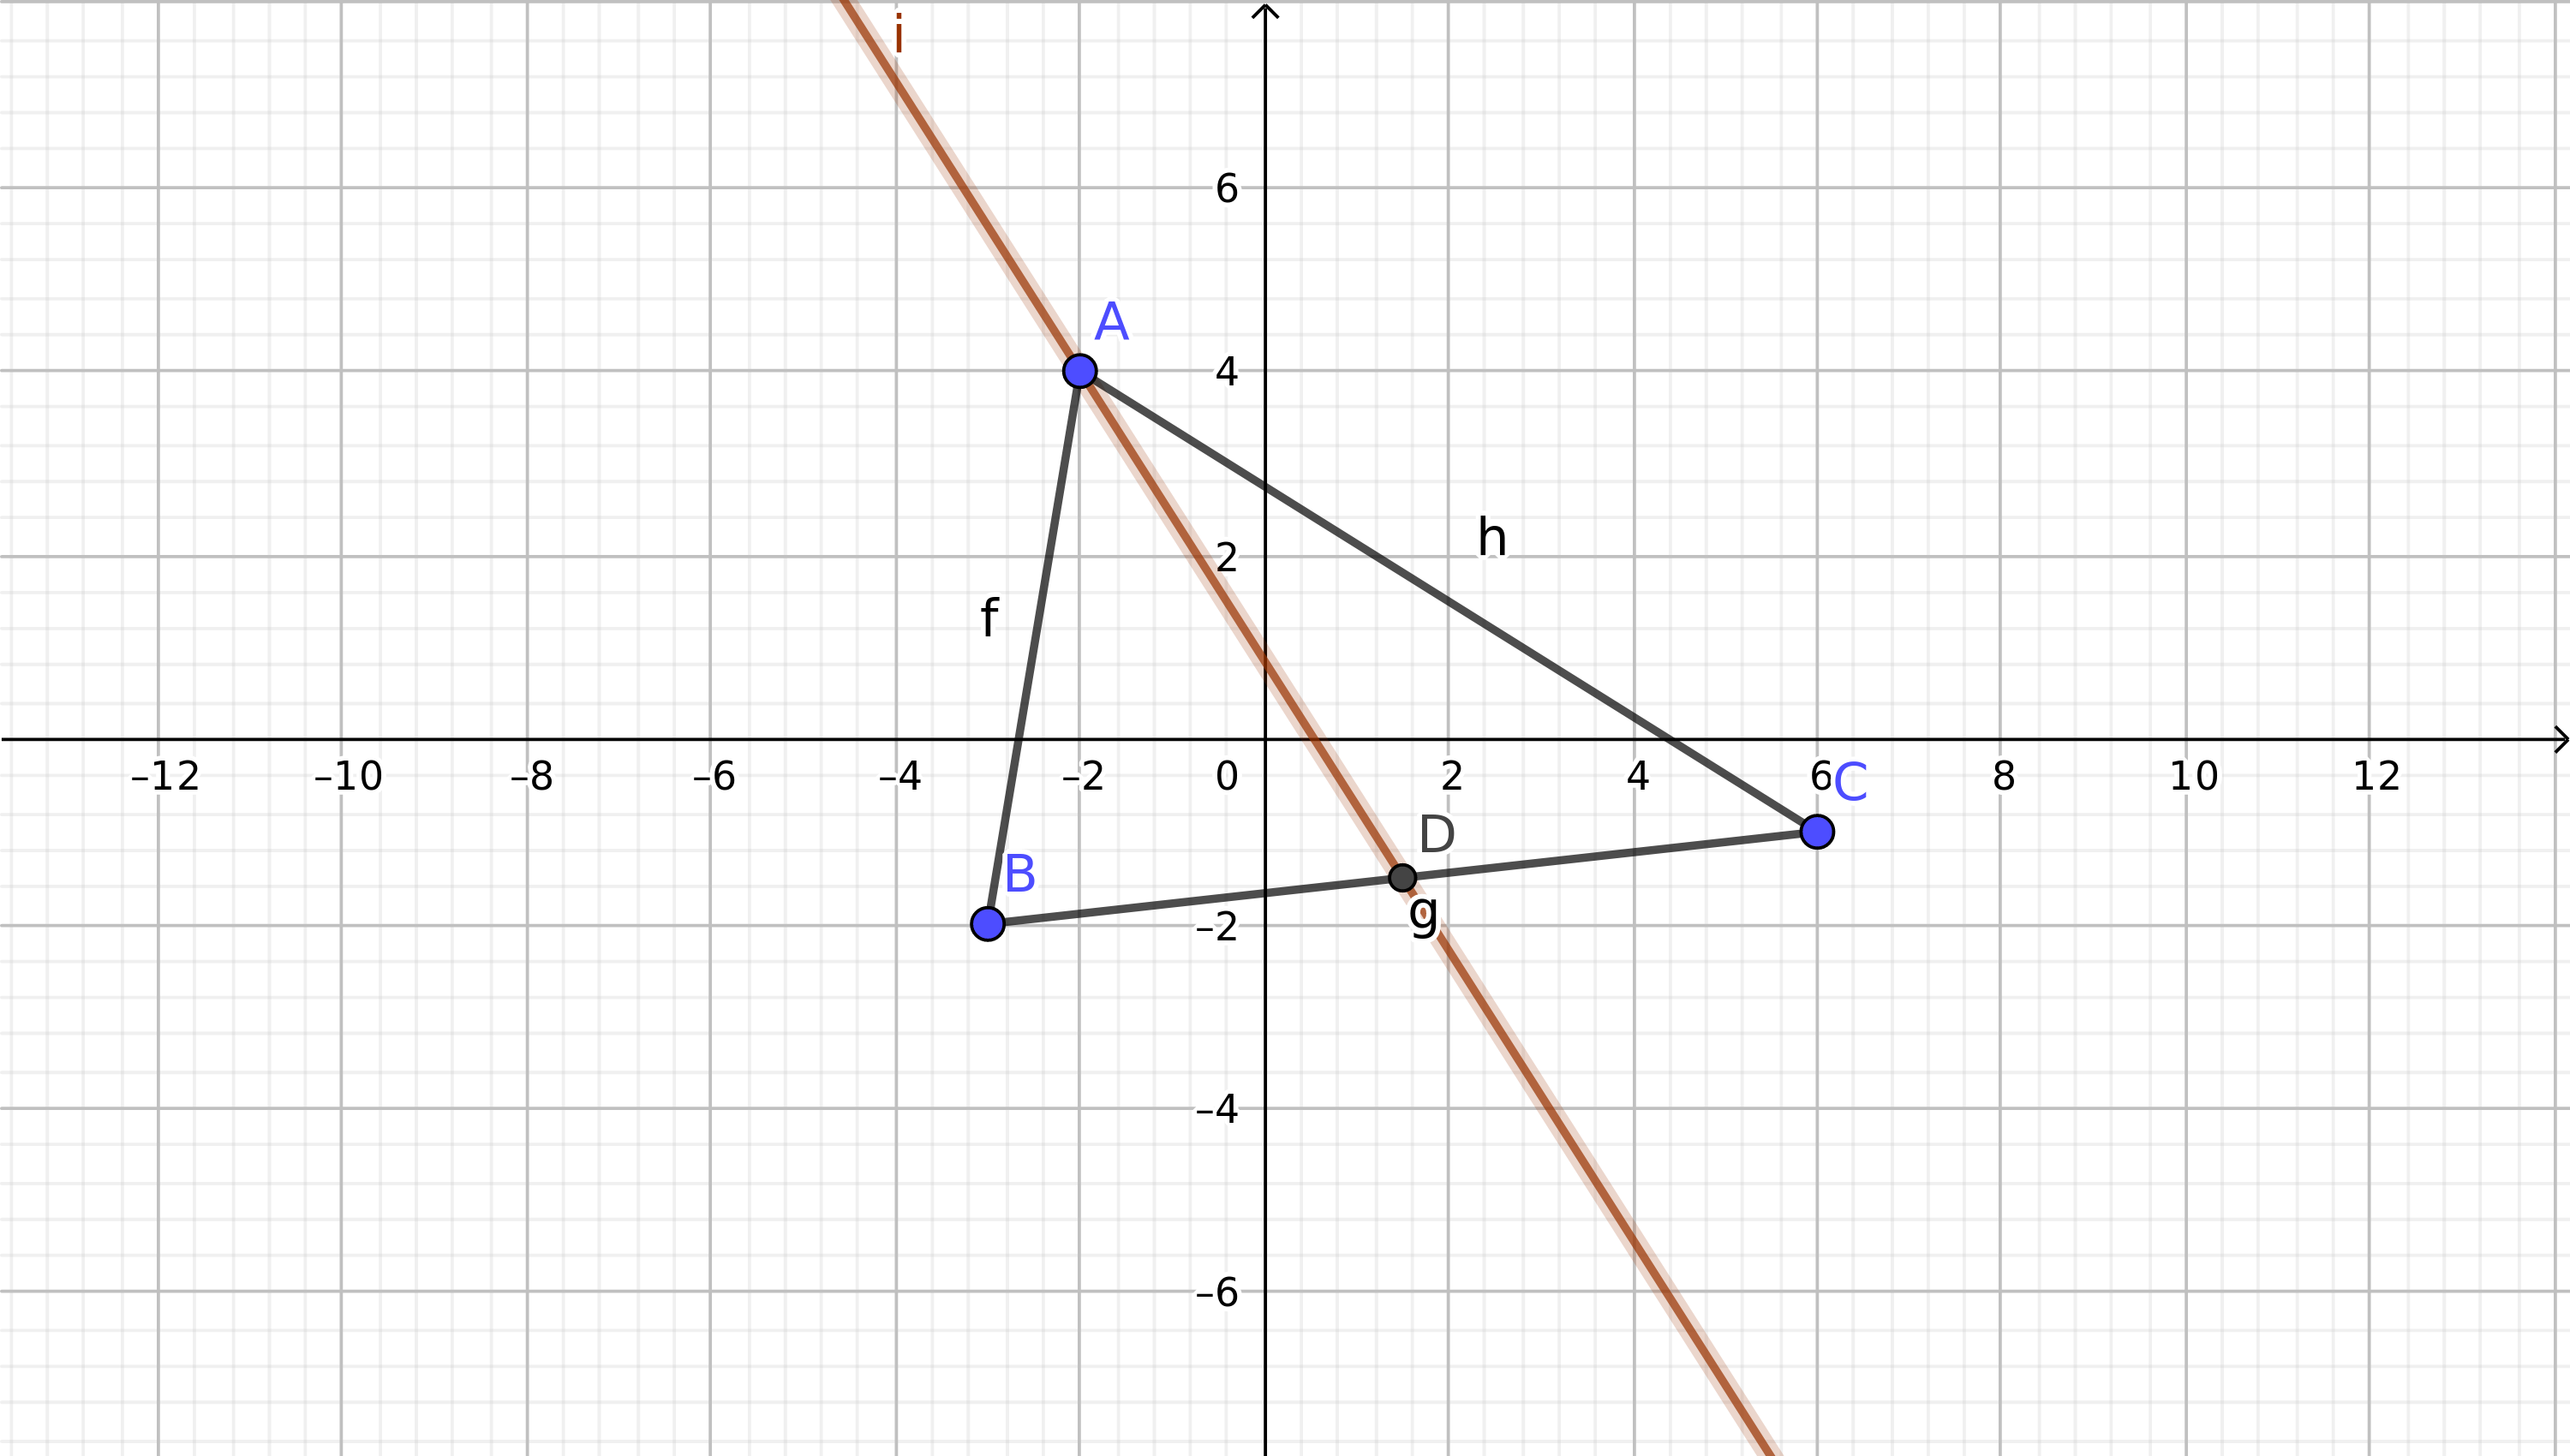
\includegraphics[scale=0.4]{img/mediana-triang.png}
\caption{La mediana que pasa por $A$, pasa por el punto medio del lado opuesto.}\label{fig:mediana}
\end{figure}

Las \emph{tres} medianas se intersecan en un punto, llamado \textbf{\color{purple}baricentro}, el \emph{\color{purple}centro de gravedad} del triángulo.

Las coordenadas del punto medio $D$ del segmento $\overline{BC}$ son las \emph{\color{purple}medias aritméticas} de las coordenadas de los extremos del segmento, de $B$ y de $C$,
\begin{equation*}
D=(d_1,d_2)=\left(\frac{-3+6}{2},\frac{-2+(-1)}{2}\right) =\left(\frac{3}{2},-\frac{3}{2}\right).
\end{equation*} 

La mediana buscada pasa por los puntos $A$ y $D$, su pendiente es la razón de los incrementos $\Delta y$ y $\Delta x$.
\begin{equation*}
\Delta y = -\frac{3}{2}-4 = -\frac{11}{2}\,,\qquad
\Delta x = \frac{3}{2}-(-2) = \frac{7}{2}\,.
\end{equation*}
Luego
$$m=\frac{\Delta y}{\Delta x} = \left. -\frac{11}{2}\Bigm/\frac{7}{2}\right. = -\frac{11}{7}.$$

Para completar la forma canónica de la ecuación de la mediana que pasa por $A$ falta hallar $b$
$$y=-\dfrac{11}{7}x+b.$$

Substituimos en la ecuación anterior las coordenadas de $A$ y obtenemos
$$4=-\dfrac{11}{7}(-2)+b,\quad\text{de donde}\quad b=4-\frac{22}{7}=\frac{6}{7}.$$
Así, la ecuación buscada de la mediana, en su forma canónica, es
$$y=-\dfrac{11}{7}x+\frac{6}{7}.$$

Verifica que la forma general de la ecuación es $5{.}5x+3{.}5y=3$.

¿Puedes encontrar el \textbf{\color{purple}baricentro del triángulo?}





\fej
\vfill 

\begin{center}
	{\footnotesize\color{olive} Hoja formada con \LuaLaTeX. La gráfica con \textsc{Geogebra}, \url{https://www.geogebra.org/}}
\end{center}


\end{document}

\begin{align*}
	\left(\frac{-4}{17}-\frac{11}{17}\right)x&=\frac{7}{17}-\frac{6}{7}\\
	\left(\frac{-28-11\cdot17}{17\cdot7}\right)x
	&=\frac{49-6\cdot17}{17\cdot7}\\
	x&=\left(\frac{49-6\cdot17}{17\cdot7}\right)\left(\frac{17\cdot7}{-28-11\cdot17}\right)\\
	x&=\frac{49-6\cdot17}{-28-11\cdot17}
	.
\end{align*}